\chapter{Desarrollo del Proyecto}
En este capítulo se discute sobre el trabajo a realizado para la completitud del proyecto, así como la descripción y el post-mortem de las diferentes actividades realizadas durante su realización.

\section{Producto propuesto}
El producto desarrollado fue un videojuego multi-jugador donde los alumnos puedan aprender conceptos básicos de los lenguajes de programación, viendo los conceptos de programación estructurada, mediante acertijos que les permitan de otra manera analizar su funcionamiento. Este se enfoco en la enseñanza de: variables, condicionales, ciclos y funciones. Estos tratarán temas de programación estructurada, basado en el material del curso de Fundamentos de la Programación y Programación I de la Universidad Autónoma de Ciudad Juárez, así como los libros Fundamentos de programación: Algoritmos, estructura de datos y objetos de Luis Joyanes Aguilar y Prelude to Programming: Concepts and design de Steward Venit y Elizabeth Drake. 
Las mecanicas del juego fueron inspiradas en el videojuego \textit{Among Us}. En este juego, un grupo de máximo 10 jugadores están juntos en una partida, hay una variedad de mapas y el punto es realizar todas las actividades que tienen asignadas para ganar. Pero del grupo unos cuantos son asignados como impostores y su trabajo es matar a los demás jugadores, sin embargo, los jugadores pueden reportar muertes o sonar una alarma que les permite discutir y votar por quien es impostor, si sacan a todos los impostores, ganan los \textit{crewmates}, los jugadores no impostores.
El videojuego tendrá una duración aproximada de 20-30 minutos.

\section{Forma de validación}
Para la evaluación de la eficacia de este videojuego en la enseñanza de programación se realizarán pruebas con dos grupos con alumnos del campus de Ciudad Universitaria de la UACJ.
Estas dos clases tendrán alumnos totalmente distintos. Estas se realizarán de la siguiente manera:
\begin{itemize}
    \item En la primera clase se colocaron a los alumnos en un lobby del producto esperado y tendrán que completar una partida del videojuego con todos los puzzles, se resolverán dudas que los participantes hagan, pero en general todo estará relacionado al juego.
    \item La segunda y similar en tamaño, fue una clase de dos horas aproximadamente donde se enseñarán conceptos de programación estructurada con Scratch, un lenguaje de programación por bloques, se separará en secciones donde cada una alberga un concepto nuevo y una pequeña actividad de 5 a 10 minutos, se tendrá el mismo temario que en el videojuego.
\end{itemize}

Al terminar se les hizo un pequeño examen donde se verá el conocimiento sobre los diferentes temas que vieron en el juego y se comparo su rendimiento, estos dos grupos son muestras distintas de una población de todos aquellos universitarios y estas dos clases pueden tener un numero distinto de participantes, además de que se desconoce la forma en la que estarán distribuidos sus resultados, por lo que se usara la prueba de la U de Mann-Whitney, una prueba no paramétrica que permitirá hacer una afirmación sobre una hipótesis nula, en este caso si se ha encontrado mejora en el rendimiento (denotado por su resultado en el \textit{quiz}) entre los dos grupos.
Adicionalmente, el examen contará con preguntas adicionales sobre la opinión de los estudiantes sobre el método de enseñanza, tales como: si les entretuvo, si se les hizo interesante, cuanto se les hizo que aprendieron en una escala del 1 al 10, y si les intereso la programación y se realizará un análisis comparativo. 

\begin{figure}[h]
    \centering
    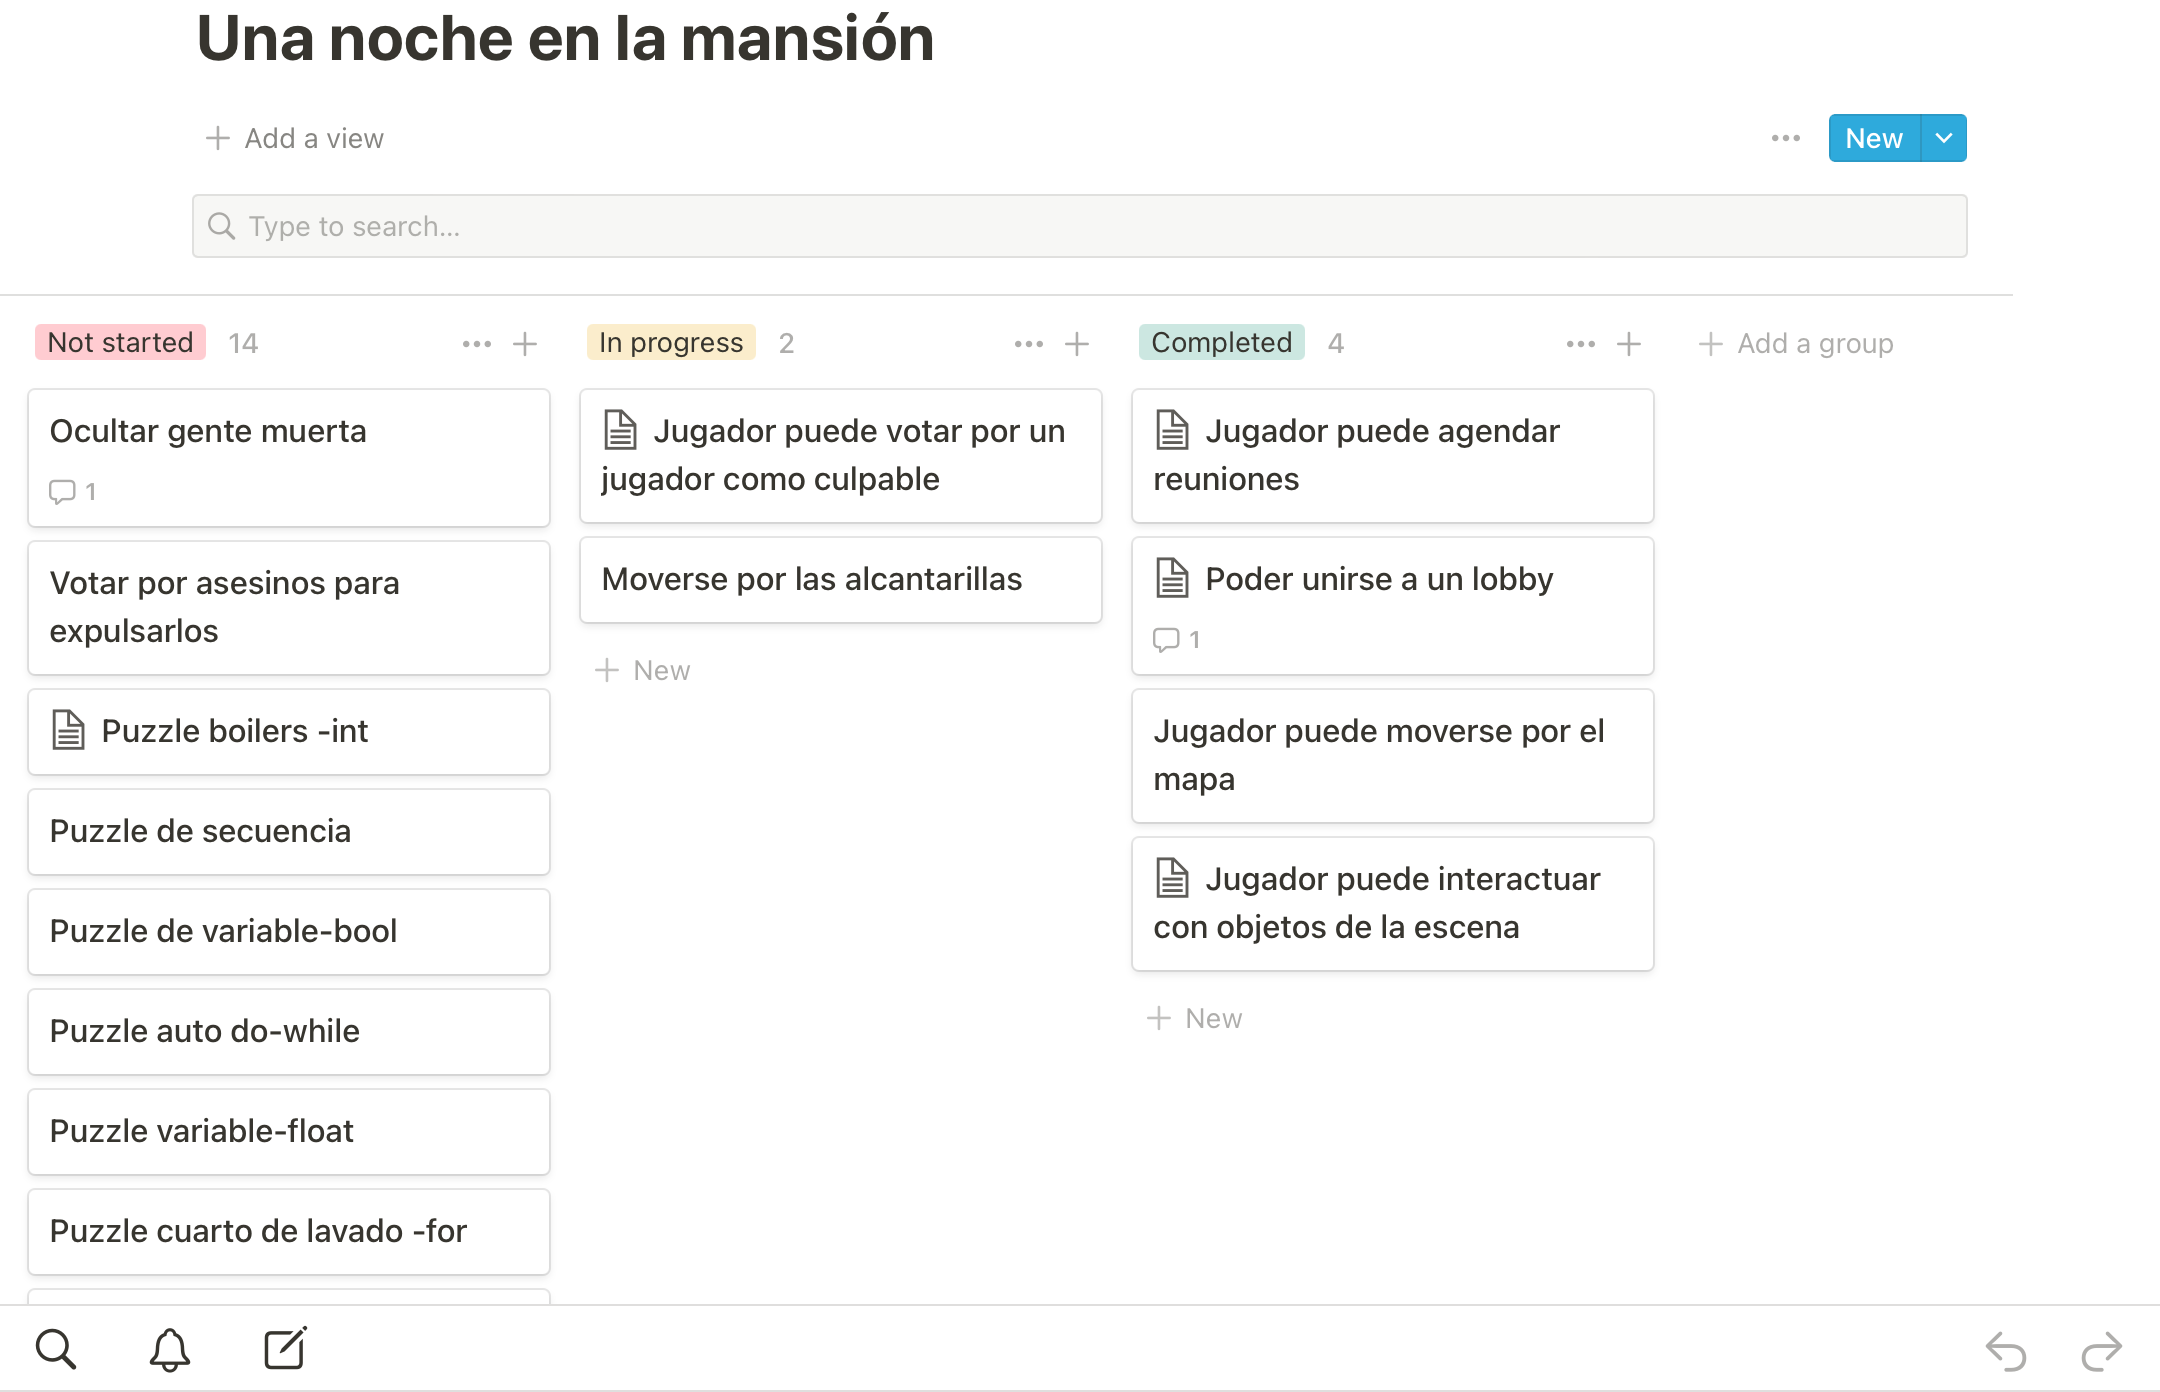
\includegraphics[width=0.8\linewidth]{images/notion.png}
    \caption{Notion con las actividades en diagrama \textit{Kanban}, en imagen nombre preliminar del proyecto}
    \label{fig:notion_proyecto}
\end{figure}

\section{Metodología}

\begin{table}
\centering
\begin{tabular}{llll}
Actividades                                         & Fecha de inicio & Fecha de termino   & Duración \\
\hline
Jugador puede agendar reuniones                    & 3-Feb-21  & 4-Feb-21  & 1      \\
Poder unirse a un lobby                            & 17-Dec-20 & 19-Dec-20 & 2      \\
Jugador puede moverse por el mapa                  & 2-Jan-21  & 2-Jan-21  & 0      \\
Jugador puede interactuar con objetos de la escena & 3-Jan-21  & 3-Jan-21  & 0      \\
Jugador puede votar por un jugador como culpable   & 24-Jan-21 & 2-Feb-21  & 9      \\
Moverse por las alcantarillas                      & 4-Feb-21  & 5-Feb-21  & 1      \\
Ocultar gente muerta                               & 5-Feb-21  & 5-Feb-21  & 0      \\
Votar por asesinos para expulsarlos                & 6-Feb-21  & 7-Feb-21  & 1      \\
Puzzle boilers -int                                & 8-Feb-21  & 8-Feb-21  & 0      \\
Puzzle de secuencia                                & 9-Feb-21  & 10-Feb-21 & 1      \\
Puzzle de variable-bool                            & 11-Feb-21 & 11-Feb-21 & 0      \\
Puzzle auto do-while                               & 12-Feb-21 & 12-Feb-21 & 0      \\
Puzzle variable-float                              & 12-Feb-21 & 13-Feb-21 &        \\
Puzzle cuarto de lavado -for                       & 14-Feb-21 & 14-Feb-21 & 0      \\
Puzzle zaguán- llenar cubeta -while                & 15-Feb-21 & 15-Feb-21 & 0      \\
Puzzle if                                          & 16-Feb-21 & 16-Feb-21 & 0      \\
Puzzle string-substring                            & 17-Feb-21 & 17-Feb-21 & 0      \\
Puzzle if/else                                     & 17-Feb-21 & 17-Feb-21 & 0      \\
Puzzle de saboteo para boiler                      & 18-Feb-21 & 18-Feb-21 & 0      \\
Puzzle para saboteo para electricidad              & 19-Feb-21 & 19-Feb-21 & 0      \\
Investigación de antecedentes                      & 12-Aug-19 & 9-Sep-19  & 28     \\
Establecimiento de objetivos del proyecto          & 9-Sep-19  & 20-Sep-19 & 11     \\
Desarrollo del marco referencial                   & 16-Sep-19 & 20-Sep-19 & 4      \\
Definición del producto esperado                   & 23-Sep-19 & 23-Sep-19 & 0      \\
Metodología de desarrollo                          & 30-Sep-19 & 4-Oct-19  & 4      \\
Cronograma de actividades                          & 30-Sep-19 & 4-Oct-19  & 4      \\
Entrega del borrador final                         & 16-Oct-19 & 16-Oct-19 & 0      \\
Presentación                                       & 17-Oct-19 & 17-Oct-19 & 0      \\
Atención a las observaciones de los asesores       & 28-Oct-19 & 13-Nov-19 & 16     \\
Presentación del desarrollo del proyecto           & 15-Nov-19 & 15-Nov-19 & 0      \\
Redacción del capítulo de desarrollo del proyecto  & 17-Dec-20 &           &       
\end{tabular}
\label{table:fechas_actividades}
\caption{Actividades del proyecto}
\end{table}

La metodología de desarrollo de software usada fue Kanban. Para la organización del tablero usamos \textit{Notion} (figura~\ref{fig:notion_proyecto}) aprovechando su vista de tablero Kanban, lista de actividades y diagrama de Gantt. En los siguientes puntos a tratar se llevaron a cabo en la planeación de actividades y en cada una de las actividades a realizar y se describirá con mas detalle la realización del proyecto. En la tabla~\ref{table:fechas_actividades}, se puede ver las actividades realizadas a lo largo de la duración del proyecto. Desde las actividades del anteproyecto, definiendo el producto esperado, hasta la realización del proyecto. 

\subsubsection{Diagrama Gantt}
(Agregar pronto)

\subsubsection{Métricas de Kanban}
\begin{figure}[h]
    \centering
    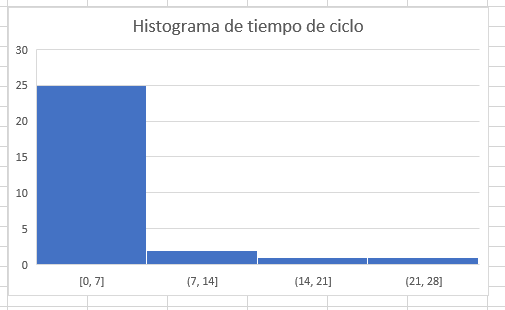
\includegraphics[width=0.8\linewidth]{images/cycle_time_histogram.png}
    \caption{Gráfica de distribución de tiempos de ciclo (o \textit{Lead Time})}
    \label{fig:lead_time_histogram}
\end{figure}

Cómo anteriormente se había tratado, el tiempo de ciclo o \textit{Lead Time} es el tiempo de realización de la tarea, abarca desde que se empieza a trabajar hasta la completitud de la tarea. Por lo general, es bueno cuando el tiempo de ciclo es corto porque significa que no hay obstáculos que el equipo de trabajo necesite sortear. De manera similar, como se nota en la figura~\ref{fig:lead_time_histogram} la mayoría de las actividades fueron resueltas en corto tiempo, la única excepción fueron actividades donde surgieron problemas técnicos no esperados, los \textit{unknown unknowns}. El principal motivo de estos fue el uso de \text{Mirror} que aumento la complejidad por la sincronización entre el cliente y la documentación de la librería es muy escasa arriba de la configuración básica, incluso considerando la de su antecesora Unet.

\subsection{Análisis}
\subsubsection{Propuestas de producto}
Durante la definición del proyecto empezó la pandemia del COVID-19, ante la necesidad de el aislamiento mucha gente recurrió a una gran variedad de juegos para ocupar su tiempo libre, entre estos hubo algunos juegos que ocuparon la consciencia colectiva por al menos un rato, juegos como \textit{Animal Crossing}, \texit{Fall Guys} y \textit{Among Us}. En el caso de este ultimo, la mayoría del público lo descubrió en \textit{streams}, gente jugando con sus amigos transmitido en tiempo real, estos normalmente jugaban el juego mientras estaban en videollamada, en cierta forma simulando su inicio como juego con partidas en Red Local. Un juego con ventajas similares funciona tanto en un entorno en linea así como en un salón de clases y tiene utilidad como actividad integradora porque naturalmente hace que entre compañeros hablen y permite conocer a otras personas.
En su parte, se definió de la creación del juego en el que el usuario pueda aprender programación junto con sus compañeros, de especial importancia durante el tiempo de realización de este proyecto donde estaba activa la pandemia del COVID-19 que obligo a muchos estudiantes a tener clases a distancia. Ante esto, de preferencia que el juego fuera accesible en una multitud de dispositivos, a fin de que una gran variedad de estudiantes puedan acceder con su dispositivo o un dispositivo de la institución para participar en la actividad. Con este factor se considero la necesidad de crear un juego para navegador como producto final. A base de la experiencia previa, así como sus plataformas soportadas y su facilidad para el desarrollo se decidió usar \textit{Unity} como motor gráfico.

\section{Diseño}
\subsection{Documento de diseño}
Se trabajó en un documento detallando los diferentes sistemas del juego. En este se definieron aspectos del juego como los diferentes puzzles como ejercicios de programación que tendrá que realizar el jugador para avanzar en el juego, el arte del juego, habitaciones, mecánicas, etc.

\subsubsection{Puzzles}
\begin{figure}[p]
    \centering
    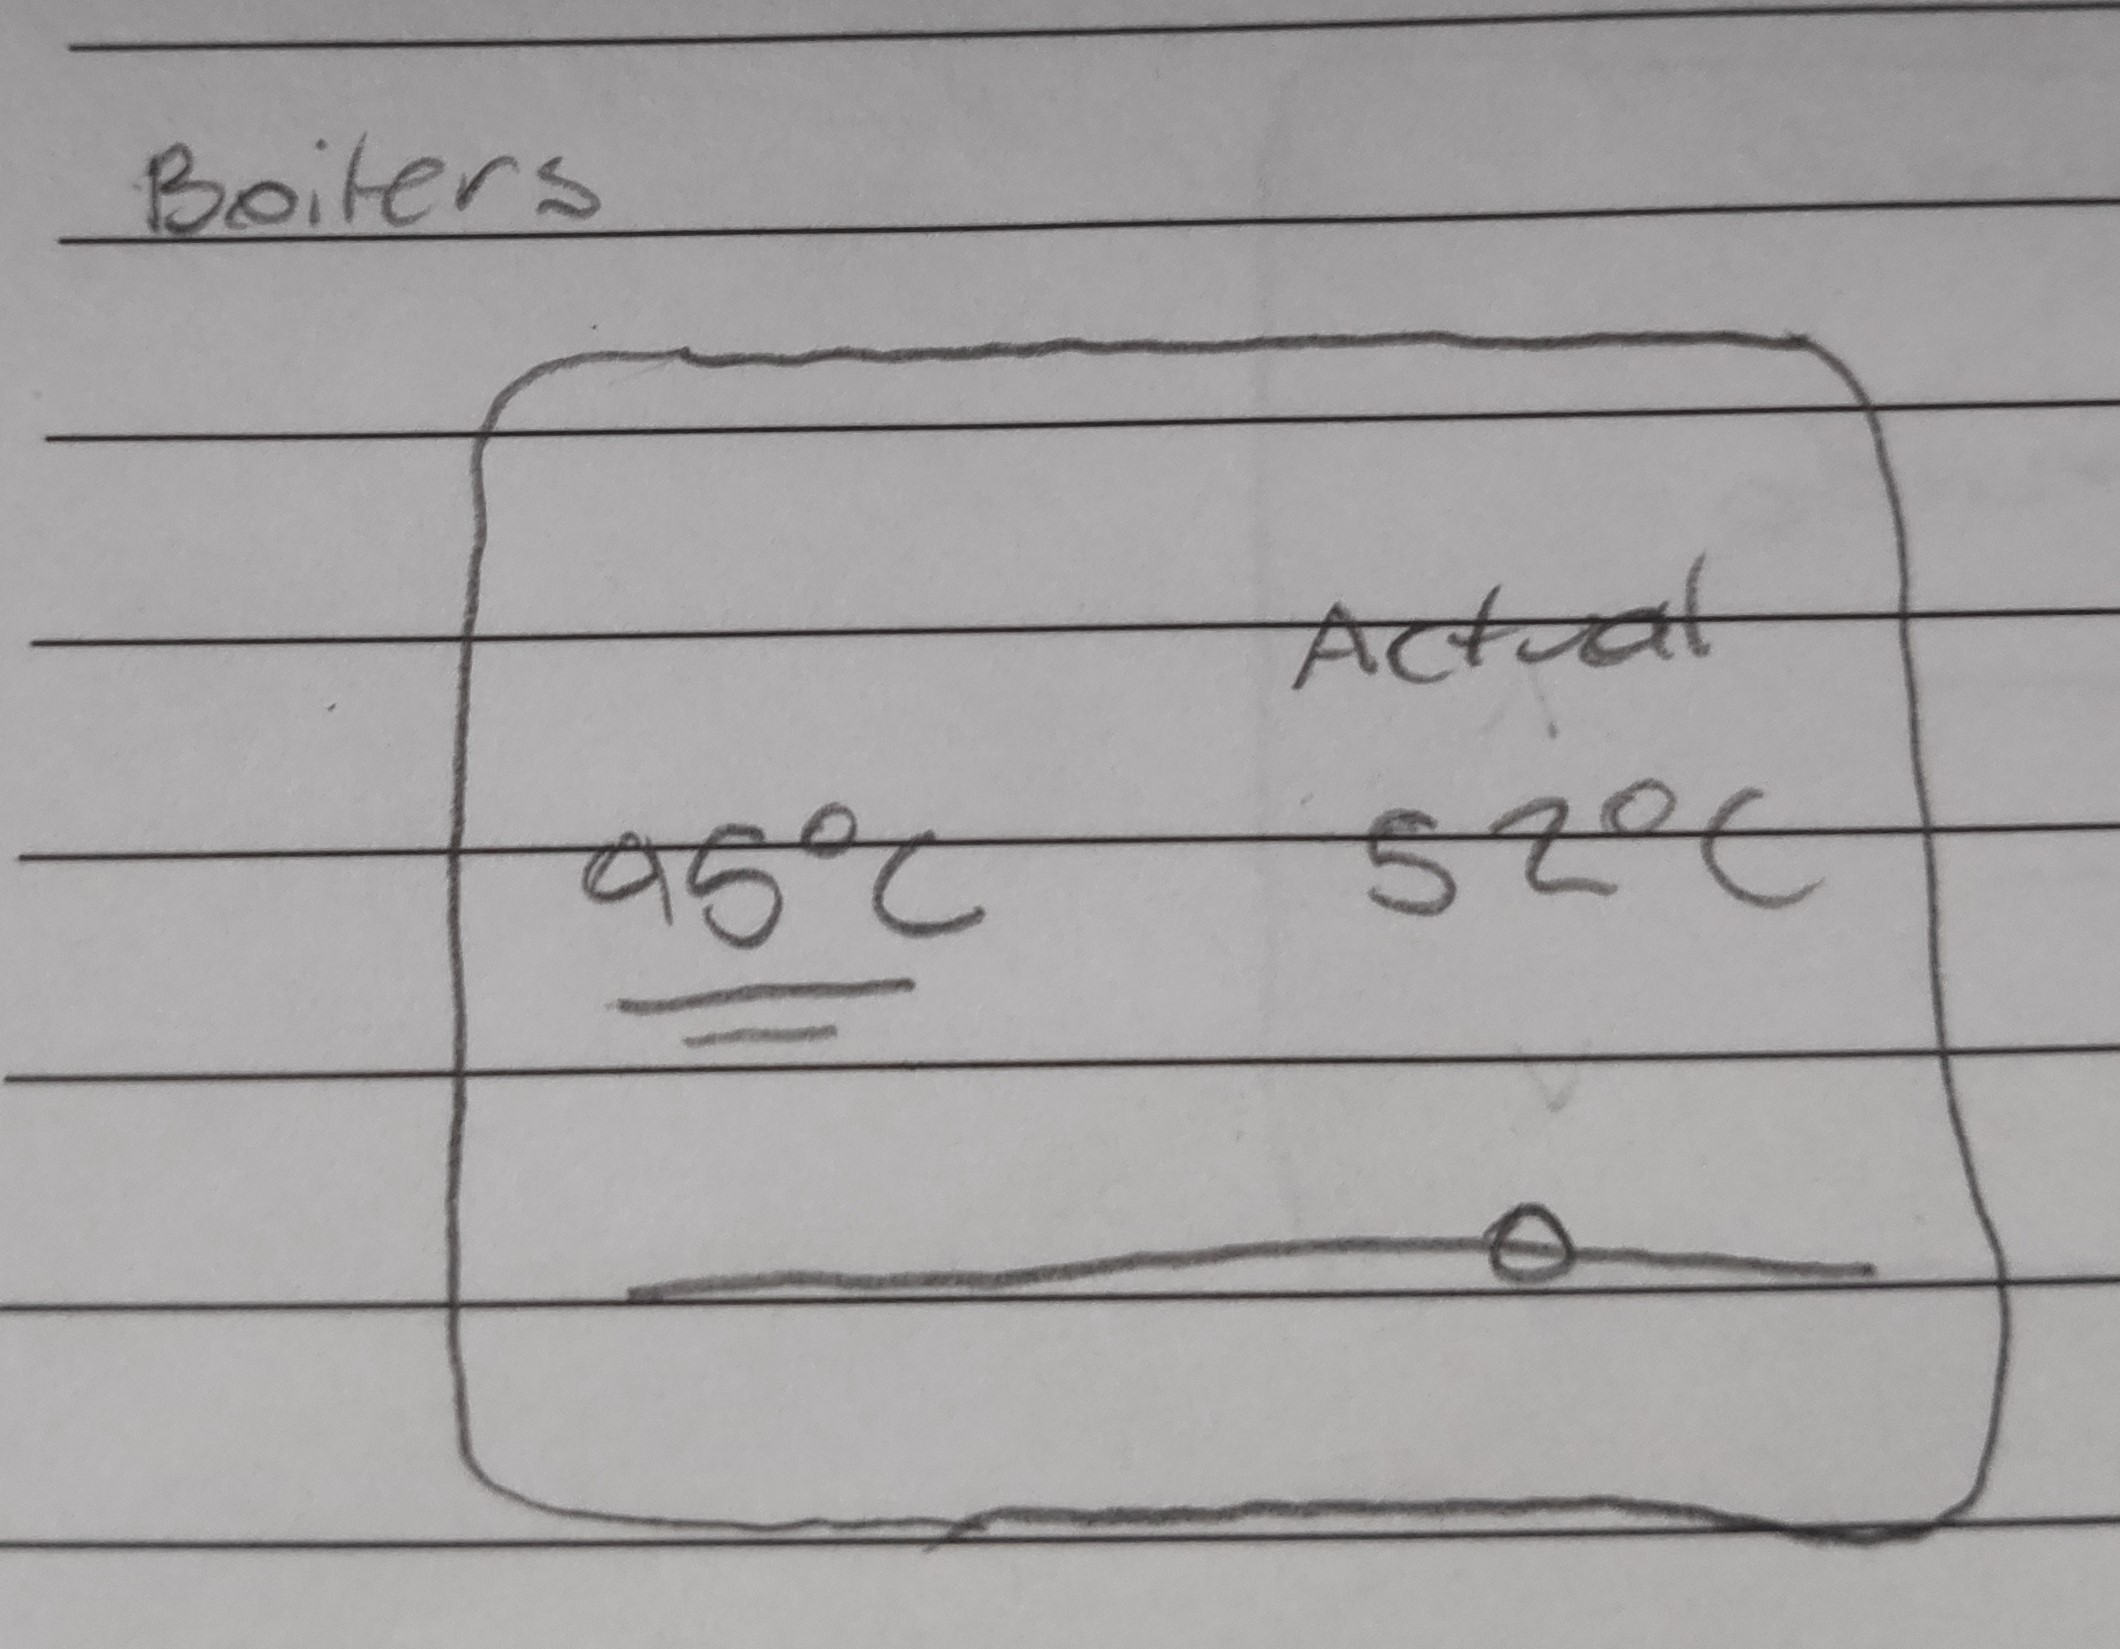
\includegraphics[width=0.5\linewidth]{images/boilers_puzzle.jpg}
    \caption{Puzzle de números enteros}
    \label{fig:puzzle_enteros_boiler}
\end{figure}
\begin{figure}[p]
    \centering
    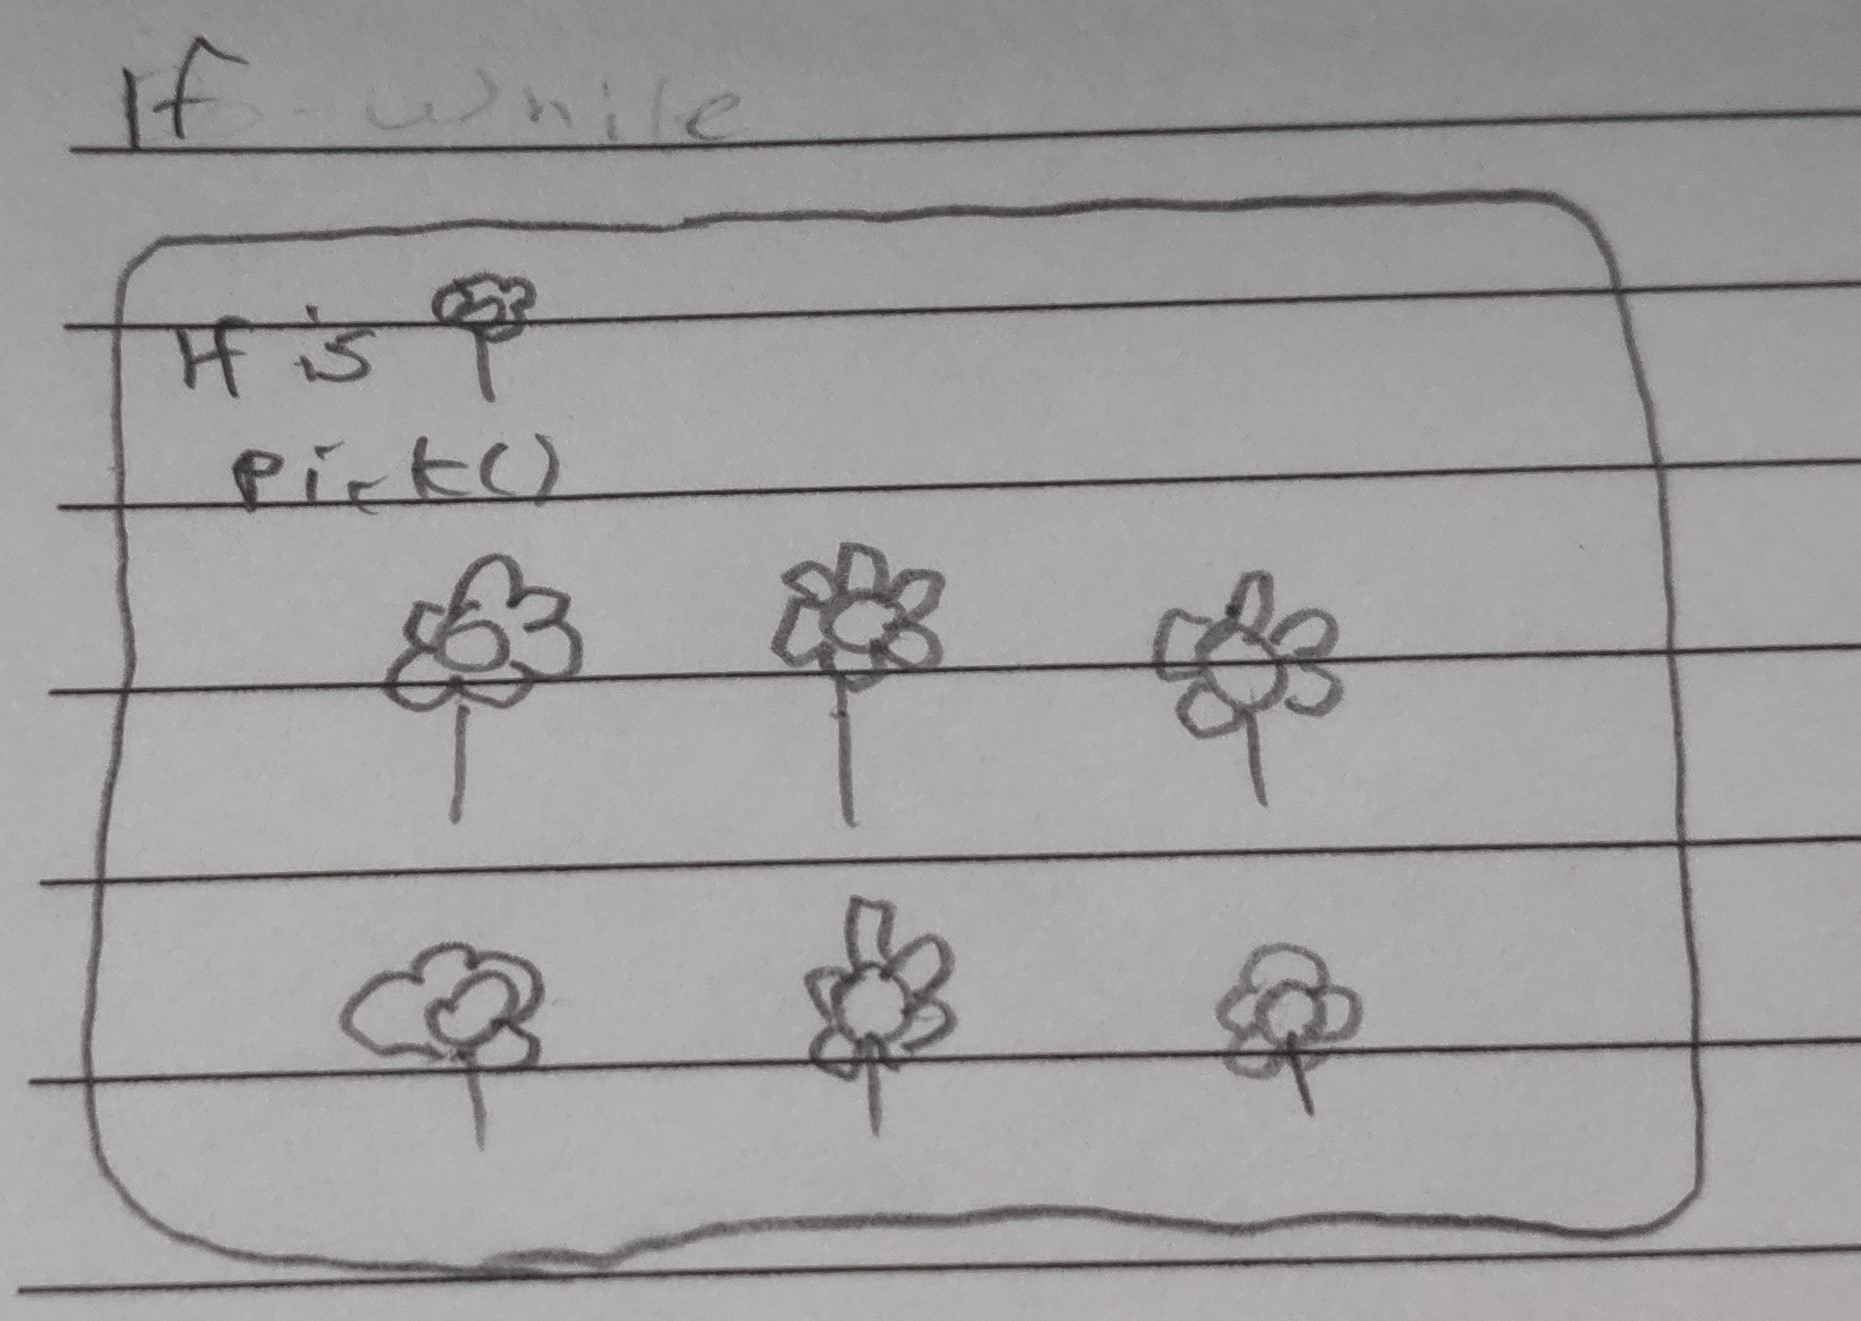
\includegraphics[width=0.5\linewidth]{images/if_puzzle.jpg}
    \caption{Puzzle de seleccionar flor, usa selección para enseñar el uso del if}
    \label{fig:puzzle_if}
\end{figure}
\begin{figure}[p]
    \centering
    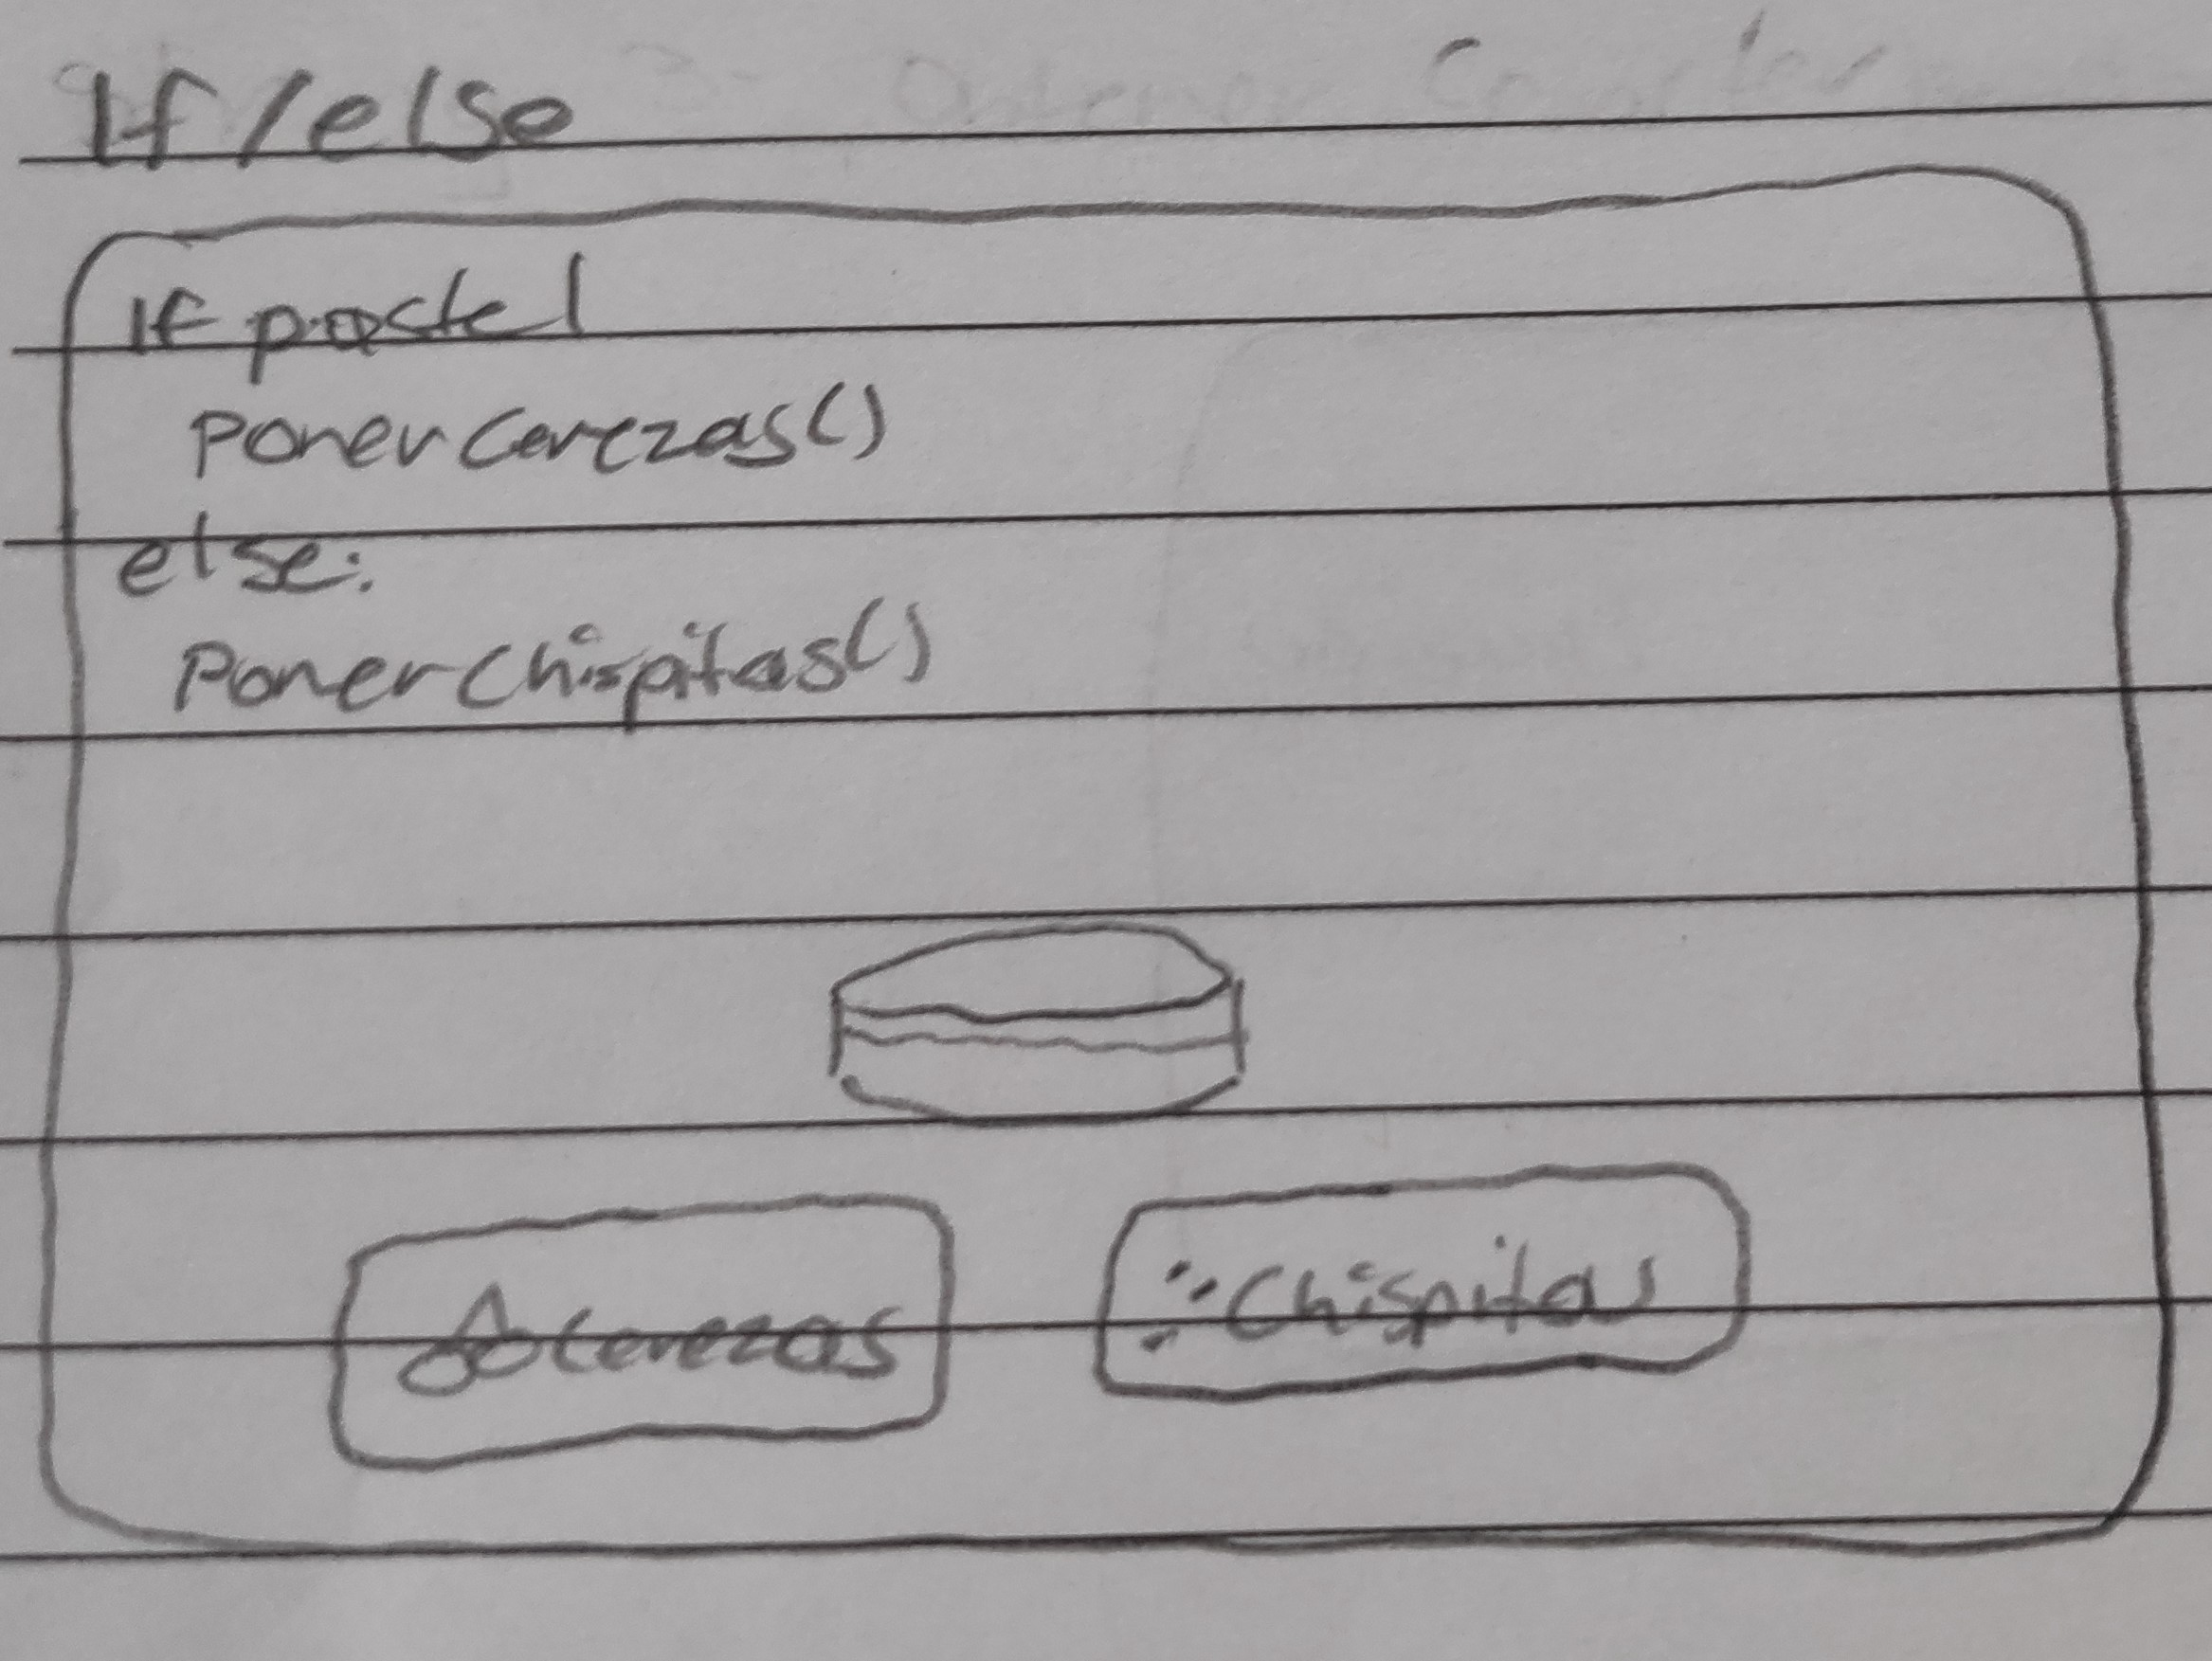
\includegraphics[width=0.5\linewidth]{images/if_else_puzzle.jpg}
    \caption{Puzzle diseñado para el if/else}
    \label{fig:if_else_puzzle}
\end{figure}

\begin{figure}[p]
    \centering
    \includegraphics[width=0.5\linewidth]{images/puzzle_while.jpg}
    \caption{Puzzle de while}
    \label{fig:while_puzzle}
\end{figure}

Los puzzles del juego fueron pensados para traer analogías del mundo real para explicar el funcionamiento de los diferentes conceptos a tratar. Con la limitante que el juego esta orientado en Inglaterra en la tarde época victoriana, cuando invenciones como la electricidad fueron utilizadas.
Para cubrir los conceptos de programación estructurada se crearon los siguientes \textit{puzzles}:

\begin{itemize}
    \item Variables tipo enteras: Con un cuarto de boilers en un extremo de la casa para brindar agua caliente, el jugador ajusta la temperatura a la que marca el termómetro, como se puede ver en la figura figura~\ref{fig:puzzle_enteros_boiler}. El puzzle se completa si el usuario mueve el \texit{slider} a la temperatura correcta.
    \item Secuencia: Entrena al jugador en su lógica de programación. Resolverlo requiere usar los cursores para moverse, requiere considerar el camino a tomar para llegar al otro lado. Cuenta como completado cuando el jugador se haya desplazado hasta el otro extremo de campo de juego del puzzle.
    \item Variables tipo string: El jugador teclea su nombre, al finalizar, un robot de servicio mostrara una caja de dialogo diciéndole Hola Juan, por poner un ejemplo. El motivo de esto es que normalmente las variables string contienen información a imprimir en pantalla y requieren operaciones como concatenación para tenerla en el formato adecuado.
    \item  Variables tipo booleano: Este tipo de variables son representadas como un \textit{switch} o un \textit{checkbox}. En este caso el jugador tendrá que volver a encender el generador moviendo la palanca. Un click mueve la palanca de una posición a la siguiente.
    \item Do While: Un do while es útil cuando la tarea a realizar requiere hacer algo al menos una vez, en este caso usamos la palanca de arranque de un automóvil que puede requerir una vuelta o unas cuantas y cuando se inicia, se tiene que alejar la mano o en la vida real uno se puede lesionar por la fuerza del motor.
    \item Variable de punto flotante: Un termostato mas avanzado en los boilers.
    \item Ciclo tipo for: Antes con el uso masivo del jabón en la época victoriana se invento el agitador, a forma de reducir el trabajo necesario para limpiar la ropa, que en lugar de tallar a mano, usa la inercia del agua para mover toda la carga y ese movimiento saca la suciedad, algo similar a las lavadoras modernas. Igual que las lavadoras, se pudiera resumir limpiar la ropa en un numero x de vueltas del agitador.
    \item Ciclo tipo while: Una cubeta requiere cierta cantidad de esfuerzo cuando se llena de en un pozo, si se tiene una bomba, requiere bombear hasta cierto punto, o si no se tira el agua de la cubeta. Este concepto permite realizar una acción monitoreando mediante una condición el nivel de la cubeta y así detenerse (figura~\ref{fig:while_puzzle}).
    \item If: Los jugadores tendrán que seleccionar la flor del tipo correcto a poner en el florero, como se nota en la figura~\ref{fig:puzzle_if}.
    \item If/else: Una versión extendida del if, en caso que no se cumpla la condicional, hay una alternativa. Haciendo alucion a la figura~\ref{fig:if_else_puzzle}, este consiste en la decoración de repostería que se lleva a cabo en la cocina, en ese día se prepararon \textit{cupcakes} y pasteles, y como se nota en el jugador sera presentado el algoritmo y a base del sprite (pastel o cupcake) tendrá que elegir la forma correcta de decorarlo. Las opciones serán mostradas como botones.
\end{itemize}

\subsection{Diseño del sistema}
\begin{figure}[h]
    \centering
    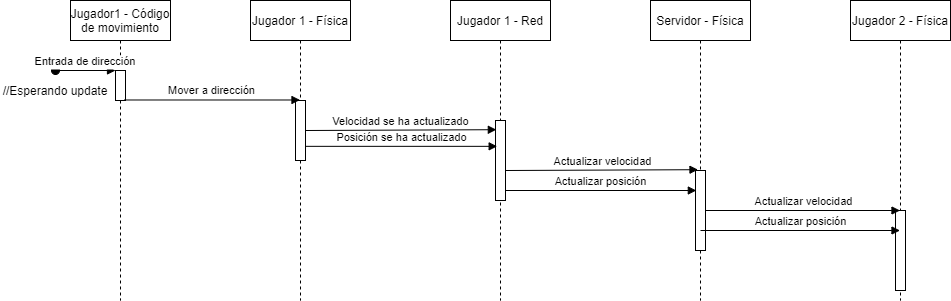
\includegraphics[width=1\linewidth]{images/diagrama_secuencia_movimientos.png}
    \caption{Diagrama de secuencia de los controles del jugador}
    \label{fig:diagrama_sec_movimiento}
\end{figure}
\begin{figure}[h]
    \centering
    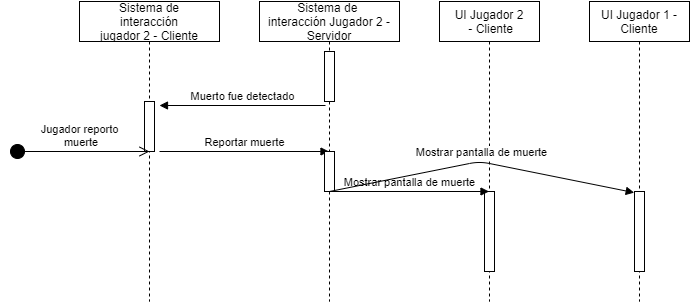
\includegraphics[width=1\linewidth]{images/diagrama_deteccion_muerte.png}
    \caption{Diagrama de secuencia de la detección de muertes}
    \label{fig:diagrama_sec_detect_muertes}
\end{figure}
\begin{figure}[h]
    \centering
    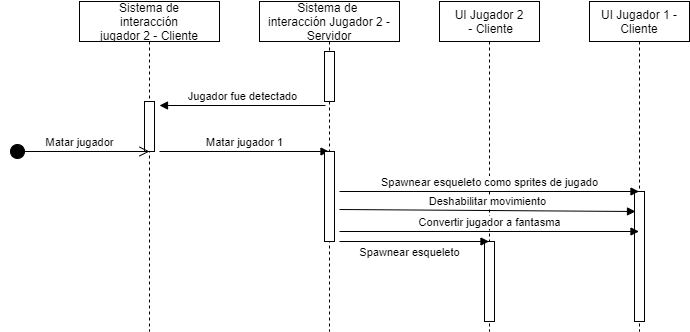
\includegraphics[width=1\linewidth]{images/diagrama_sec_matar.png}
    \caption{Diagrama de secuencia de muertes por asesinos/impostores}
    \label{fig:diagrama_sec_muertes_por_impost}
\end{figure}

En primera instancia, para el multijugador se decidió utilizar la librería \textit{Mirror} para desarrollar el sistema de multijugador. Esto es esencial, porque sus abstracciones para el manejo de las comunicaciones cliente-servidor mediante \textit{Remote Call Procedure} dictaron algunas decisiones de arquitectura.
Se diseño con un servidor autoritativo. Las acciones del jugador van al servidor para ser verificadas. Una excepción es el sistema de movimiento de los jugadores, como trataremos a continuación.como se puede ver en la figura~\ref{fig:diagrama_sec_movimiento}, en este caso cada "propietario" de su personaje tiene capacidad total de moverlo a donde quiera, en teoría. En practica, el cliente controla la posición a base de la entrada del jugador y usando sincronización de posición y velocidad de Mirror tenemos un pseudo sistema de predicción de su siguiente movimiento para conexiones lentas. 

\subsubsection{Sistema de detección de muertes}
Es un sistema que funciona primordialmente en el servidor, se puede notar su funcionamiento en la figura~\ref{fig:diagrama_sec_detect_muertes}. En todo momento, cada \textit{game loop} corre una rutina que realiza \textit{raytracing} al área circundante al jugador con un radio definido previamente en el \textit{lobby} del juego. Al haber un cambio se mandara una llamada a un procedimiento en el cliente que actualizara la interfaz gráfica para mostrar un botón de reportar muertos. Una vez al ser reportado, se realizara una segunda revisión de que sea una operación legal y se pide a todos los clientes mostrar una UI para realizar la votación sobre el personaje de juego.

\subsubsection{Asesinatos}
Hay un tipo de jugadores especiales llamados asesinos, estos son impostores que engañan a los demás jugadores de su verdadera identidad. Estos tienen entre una de sus capacidades matar a otros jugadores. El asesinar a otros jugadores es una actividad que es controlada autoritativamente por el servidor.
Como se nota en la figura~\ref{fig:diagrama_sec_muertes_por_impost}, el detectar jugadores ocurre en el servidor. En el cliente el jugador impostor puede matar a otros jugadores no impostores, cuando se manda la señal de matar a alguien (invocada por un botón) en el servidor se procesa si es legal, o sea si es físicamente posible su ocurrencia. Si es legal, se mandan funciones RPC al jugador recién muerto para que \textit{spawnee} un esqueleto en su lugar y para mandarlo a otro \textit{layer} que no es visible por los jugadores vivos (y mostrar en la cámara del juego la capa de fantasmas). En el caso del jugador 2, y la mayoría de los jugadores vivos, solo recibirán por parte del servidor un mensaje para \textit{spawnear} un nuevo \textit{sprite} del esqueleto.

\subsection{Teletransporte}
\begin{figure}[h]
    \centering
    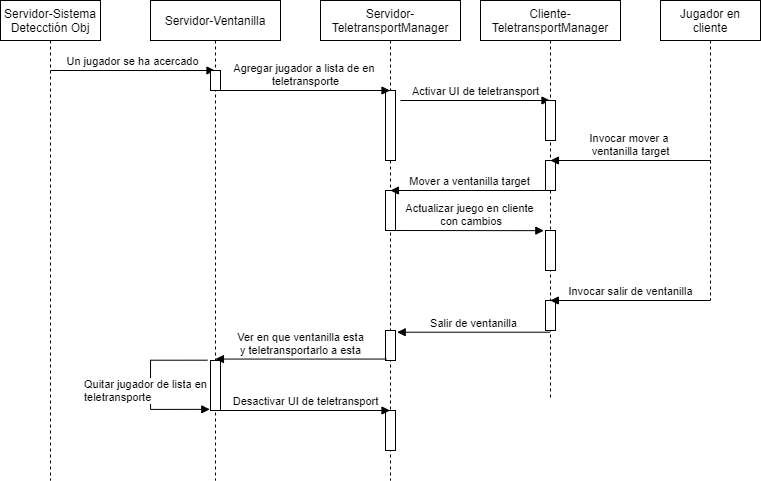
\includegraphics[width=1\linewidth]{images/DiagramaSecuenciaTeletransporte.png}
    \caption{Diagrama de secuencia de teletransporte}
    \label{fig:diagrama_sec_teletransporte}
\end{figure}
Solo disponibles para los asesinos. Es una forma de escapar de cuartos con puntos descubiertos. El sistema de teletransporte usara el sistema de interacción e incluye un estado especial donde los jugadores pueden moverse entre ventanillas conectadas. Las ventanillas agregan a el jugador que entro en ella a la lista de jugadores en modo de teletransportación, en este modo las opciones disponibles son moverse a la ventanilla \textit{target} y salir de la ventanilla actual, como se puede ver en la figura~\ref{fig:diagrama_sec_teletransporte}.

\subsection{Sabotajes}
Son tipos especiales de \textit{puzzles}. Tienen la misma complejidad que estos pero requieren 2 jugadores que los hagan al mismo tiempo para completarlos con éxito. Estos pueden ocurrir varias veces en la partida dependiendo de los "asesinos". Los asesinos pueden invocar los sabotajes después de un tiempo dado de que haya iniciado la partida, después de un tiempo de juntas y después de un tiempo de que los programadores completaron un primer sabotaje correctamente.

Hay tres sabotajes disponibles:
\begin{itemize}
    \item Apagar generadores, jugadores tienen que encender un generador de respaldo
    \item Mover presión de \textit{boilers}, jugadores tienen que regular la presión. Puzzle consiste en que los jugadores tienen que ver el indicador en pantalla y mantener la presión en verde, modificando el algoritmo en pantalla de forma que mantenga la presión entre el mínimo y el máximo.
    \item Sabotear telégrafo, requiere dos personas contesten preguntas. Al contestar un numero de dado de preguntas correctas resolverán el sabotaje.
\end{itemize}

\subsection{Mapa de juego}
\begin{figure}[h]
    \centering
    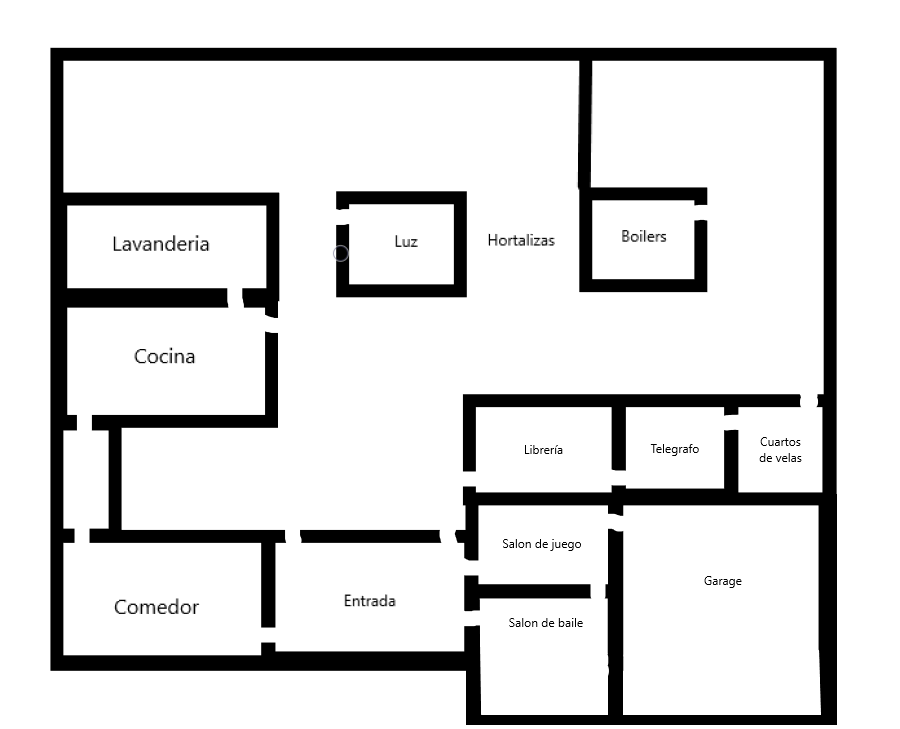
\includegraphics[width=1\linewidth]{images/MapaJuego.png}
    \caption{Organización del mapa del juego}
    \label{fig:mapa_juego}
\end{figure}
El juego se lleva a cabo en una mansión. El mapa consiste de un solo piso. Algunas de las características que se considero que tuviera el mapa fueron:
\begin{itemize}
    \item Interconectado para permitir a los programadores moverse a completar sus actividades, de preferencia mas de una salida distinta. En el caso de que el cuarto tenga varias salidas o este en un sándwich con otras habitaciones a los lados se pueden agregar opciones adicionales para los impostores como el sistema de teletransporte de manera que no se tengan que preocupar de que un programador salga de una entrada fuera de la vista del asesino y lo agarre sin manera de escapar, de manera que sea justo para los asesinos y su juego no quede a cosas fuera de su control.
    \item Hay algunos cuartos que rompen con la primera regla para los programadores, tienen una sola salida y es muy fácil de que un asesino agarre a un programador haciendo una tarea y fácilmente lo pueda matar. Dado que hay poco flujo de transito, la tumba puede quedar no detectada por un rato. La forma de balancear esto es agregando varias tareas en este cuarto de forma que otros jugadores tengan la necesidad de entrar. Algunos jugadores mas experimentados dada la reputación de esos cuartos podrán entrar a revisar si no hay ninguna tumba de alguno de sus compañeros programadores.
    \item Áreas principales grandes donde los jugadores circulan a las diferentes salas del juego, normalmente son zonas que un asesino consideraría muy alto riesgo para matar a un programador. Estas son la entrada a la mansión, un patio, el saguán de atrás de la casa y un patio que conecta los \textit{boilers} con un corral.
\end{itemize}

El diseño del mapa se puede ver en la figura~\ref{fig:mapa_juego}.

\section{Desarrollo}
Usando las libertades dadas por la librería Mirror, en el mismo proyecto de Unity se desarrollo el \textit{codebase} del cliente y el servidor, usando el lenguaje de programación C\#. El servidor se encarga de hospedar las partidas y los clientes que dependen del servidor para manejar el estado usan esta misma librería sincronizar estado además de realizar llamadas y ejecutar comandos a petición del servidor.

El juego se diseño con un servidor autoritativo, algunos sistemas hacen cálculos en el servidor y las decisiones son rectificadas también en este. En si, el estado del juego será computado mayormente en el servidor, donde el cliente solo estará como un cliente ligero. La comunicación entre estos dos se realizara con el protocolo usando \textit{Websockets} para la transferencia de información, una limitación dada por el soporte de protocolos de comunicación del navegador web.

En esta etapa se realizo la programación de diversos sistemas y comportamientos de distintos elementos del juego.

\subsection{Creación de \textit{sprites} y \textit{assets}}
Según detalles del documento de diseño, se crean los diversos sprites para elementos del
mundo como: personajes, animaciones e interfaces gráficas.

Existieron varios donde fue necesario realizar \textit{sprites} para el arte del juego. El diseño de estos artículos se realizo previamente en el documento de diseño del juego y se definieron algunas limitantes, como la resolución, donde cada \textit{tile} mide Tienen medidas de 16x16. En los \textit{sprites} necesarios, estuvieron los de personajes jugables (figura~\ref{fig:sprite_johanna}. Estos \textit{sprites} se diseñaron en \textit{Photoshop} en el caso de los jugadores miden 1x2 \textit{tiles}.

\begin{figure}[h]
    \centering
    
\includegraphics[width=0.2\linewidth]{images/JohannaOrdonez.png}
    \caption{Sprite de uno de los personajes jugables}
    \label{fig:sprite_johanna}
\end{figure}

Se encontraron \textit{spritesheets} que se pudieran usar con licencia en el proyecto en el sitio web \url{http://itch.io}, esto nos permitio reducir el trabajo de crear arte para el juego.
Entre estos fueron:
\begin{itemize}
    \item \textbf{Grass++} Variedad de sprites de pastos, flores y miscelaneos para los patios y jardines
    \item Platformer 2D Tileset
    \item Dungeon Tileset
    \item Free Tileset Objects - Treasure Chests
\end{itemize}

\subsection{Sistema de versiones}
Para la elaboración del proyecto se usó el sistema de versiones Git. El repositorio es público y puede ser accedido en \url{https://github.com/SaulNunez/Project-Hamilton}.

\subsection{Integración Continua}
Se usó Github Actions permite ejecutar un \textit{script} después de crear nuevos \textit{commits} a la rama \textit{Master}.
Ejecuta las siguientes acciones cada vez que se activa el trabajo:
\begin{itemize}
    \item Compila ejecutables para Windows x64-86 y WebGL
    \item Crea documentación de las funciones y variables del proyecto y sube usando \textit{Github Pages} la nueva versión a la página \url{http://saulnunez.com/Project-Hamilton/}
\end{itemize}

Para la compilación de ejecutables se usó el increíble trabajo de GameCI que tiene imágenes preconfiguradas de Unity que facilitan la creación de los \textit{pipelines} necesarios para la compilación. Se uso su tutorial disponible en \url{https://game.ci/docs/github/v1/builder} y sus ejemplos para la creación del \textit{script}.

En la creación del pipeline de la generación de documentación se usó el trabajo de Normand Erwan disponible en \url{https://github.com/NormandErwan/DocFxForUnity} que provee la configuración de DocFX para que funcione con la organización por carpetas de Unity y por la forma en la que este de manera predefinida crea clases para componentes en el \textit{namespace} \textbf{global}.

\section{Implementación}
\subsection{Sprites}
Como lo vimos anteriormente, hay dos tipos de \textit{sprites}. Aquellos que se obtuvieron de itch.io se agregaron simplemente a Unity importándolos a las carpetas del proyecto y configurado para que los interpretara como \textit{"sprites"}, estos al ser \textit{spritesheets} (y por lo tanto contener en un solo archivo un numero de \textit{sprites} individuales) se cortan en el editor de \textit{sprites} dependiendo del tamaño en el que fueron diseñados (normalmente 16x16 o 32x32 píxeles); normalmente aquí acabaría el proceso pero en algunos sprites requirieron ajustes manuales por su forma de \textit{"sprite packing"} (como se organizan los sprites entre el archivo de imagen). En el segundo tipo, fueron los creados específicamente para el juego, estos fueron diseñados en Photoshop, se uso el \textit{plugin} de PSDs para permitir importar archivos de Photoshop directamente a Unity para utilizarlos, dependiendo de la situación del \textit{sprite} en particular se dejaba en simple o en múltiples, estos últimos cortados en  16x16 para ítems grandes que usan el principio 9-slice. 

\subsection{Despliege}
Se uso dos servicios de Amazon Web Services. 
Para el cliente que el corre cada usuario y accede por internet usamos S3.
Para el servidor se uso el \textit{trim} gratis de AWS EC2. Este fue configurado para correr Windows Server 2019, la configuración se llevo a cabo según \href{https://mirror-networking.gitbook.io/docs/guides/server-hosting/aws}{las guías de Mirror}.

(Meter diagramas de configuracion del servidor, etc)

\section{Pruebas}
Durante el desarrollo se usaron pruebas * en el producto, así como pruebas de humo para revisar que las suposiciones del funcionamiento del sistema eran correctas al finalizar la codificación de cierta funcionalidad. Estas ultimas fueron hechas de manera manual donde se prueba el producto a fin de ver si el sistema funciona.

En la implementación, se realizaron pruebas de integración de manera manual a fin de detectar que se conectara correctamente el cliente y el servidor ante las diferencias de configuración entre el entorno de pruebas y el sistema final.